\documentclass[12pt,a4paper]{report}
\usepackage[utf8]{inputenc}
\usepackage[german]{babel}
\usepackage[T1]{fontenc}
\usepackage{amsmath}
\usepackage{amsfonts}
\usepackage{amssymb}
\usepackage{graphicx}
\usepackage{titlesec} 
%\titleformat{\chapter}{\bfseries\huge}{\thechapter.\quad}{0ex}{\vspace{0.1ex}}
%[\vspace{0.1ex}]%\rule{\textwidth}{0.3pt}]
\author{Fabio Greco - Franziska Theis}

\title{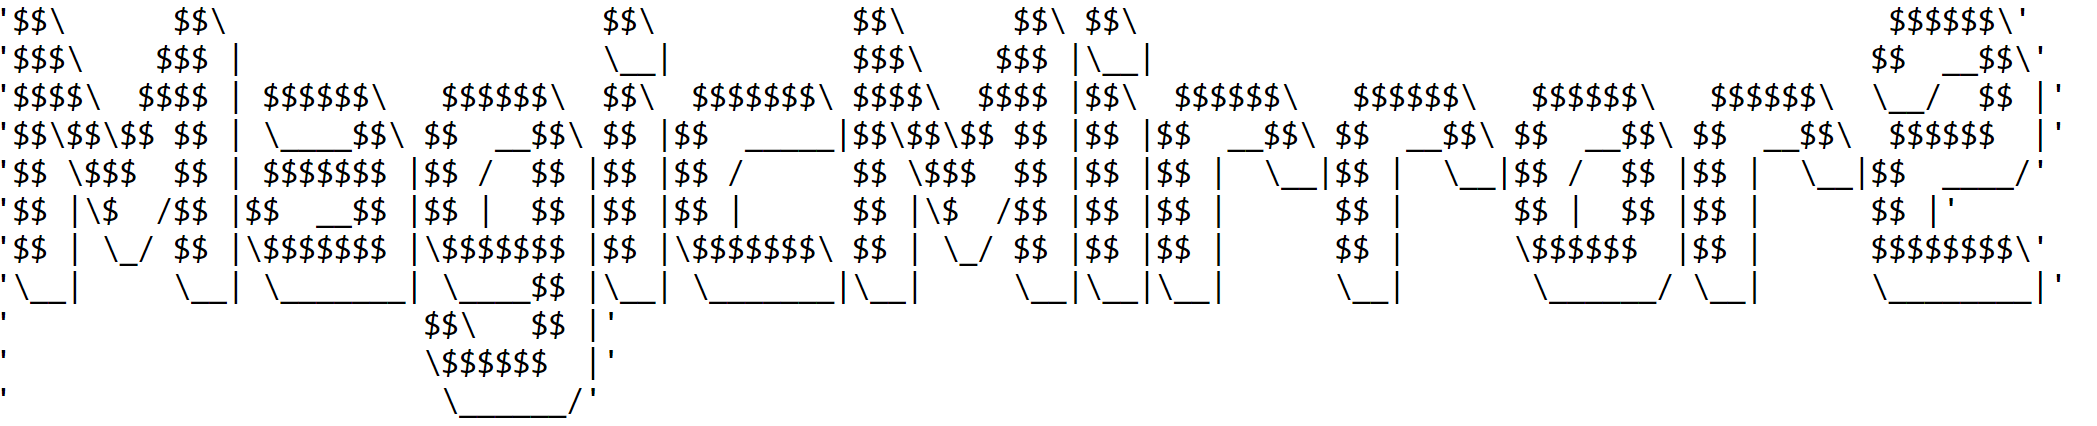
\includegraphics[scale=1]{Cover.png} \\
Implementierung eines personalisierten intelligenten Spiegels (Magic Mirror) 
}

\begin{document}
%\hspace{-50pt}
\maketitle

\chapter{Hinführung}
In Zeiten von Digitalisierung und einem ständigem Online-sein setzt das Projekt in diesem Alltag an. Ein Spiegel, der bisher nur dem Zweck diente, sich selbst darin zu sehen, wird nun erweitert. Er soll den Benutzer mit Nachrichten aus der Welt informieren, mit aktuellem Wetter auf den Tag vorbereiten und die bevorstehenden Termine bereits beim Zähneputzen anzeigen. Kurzum, der Magic Mirror, oder auch Smart Mirror genannt, soll ein Alleskönner werden. 
\section{Problemstellung}
Der Magic Mirror ist eine weitverbreitete Anwendung des Raspberry Pis, weswegen bereits mehrere Betriebssysteme verfügbar sind. Die Betriebssysteme werden später vorgestellt. 
Die Auswahl und Konfigurierung der zugehörigen Module, beispielsweise ein Kalender oder ein Newsfeed, werden ebenfalls in den weiteren Kapiteln beschrieben. 
Damit der Magic Mirror für mehrere Personen nutzbar wird, welche verschiedene Interessen haben und somit andere Module als wichtig empfinden, soll eine Personalisierung implementiert werden. Wie zwischen den Profilen gewechselt werden soll, ist nicht vorgegeben, weshalb auch hier im Laufe des Berichts mehrere Möglichkeiten evaluiert werden. 
Der Controller des Magic Mirror ist der Raspberry Pi. Bei der Ausarbeitung des Projekts sind daher einige Vorkenntnisse, sowie ein Verständnis über das Betriebssystems des Raspberry Pis unabdingbar. Deshalb wird dazu im nächsten Kapitel eine kurze Einführung gegeben.



\chapter{Ziele für den ersten Prototypen}

fa

 
\chapter{Hardware-Komponenten des Magic Mirrors}
Die folgende Grafik zeigt die Hardware-Komponenten, die es benötigt, um einen Magic Mirror zu bauen. Allerdings ist es nur ein Vorschlag und kann auch auf andere Weise realisiert werden. Zunächst wird die Steuereinheit des Magic Mirrors der Raspberry Pi vorgestellt. Danach werden die übrigen Hardware-Komponenten und deren Zusammensetzung zu einem Spiegel erläutert. 
\begin{figure}[h]
\hspace{-50pt}
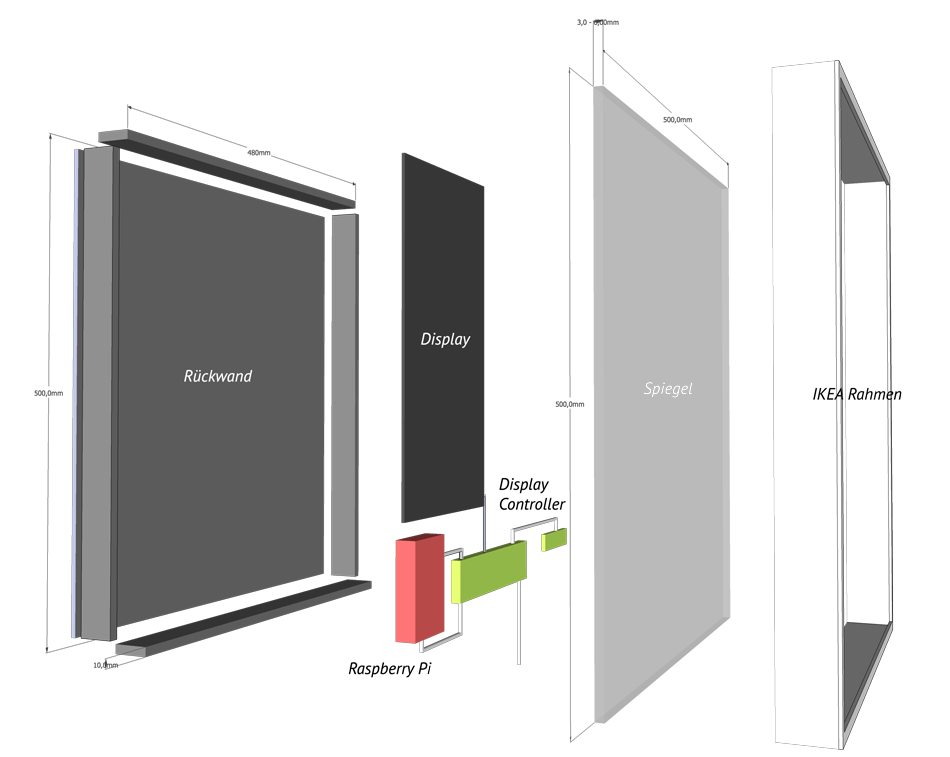
\includegraphics[scale=.5]{Bauteile.png} 
\caption{Hardware-Komponenten}
\end{figure}
\section{Raspberry Pi}
Der Raspberry Pi ist ein kompakter und günstiger aber vollwertiger Computer. Mit zahlreichen Schnittstellen und Modulen zur Erweiterung ist er sehr vielseitig einsetzbar und flexibel. In diesem Projekt wird ein Raspberry Pi 3 verwendet, das achte Modell der Reihe. Im Vergleich zu den Vorgängermodellen bringt dieser Raspberry Pi ein integriertes WLAN- und Bluetoothmodul mit. Zudem besitzt er 4 USB 2.0 Ports, einen HDMI-Anschluss, sowie einen analogen Video- und Audio-Ausgang. Sein Ethernet-Anschluss arbeitet mit 100 MBit/s. Der Prozessor nutzt vier ARMv8-Kerne. Aufgrund des verbauten Display- und Touch-Controllers kann der Raspberry Pi an ein LCD-Display oder einen Computermonitor angeschlossen werden. Über die GPIO-Leiste mit 26 GPIOs und insgesamt 40 Pins können weitere Module angesteuert werden oder Messaufgaben mit Sensoren übernommen werden. (Quelle: Heft c't Raspberry Pi Praxiswissen und Know-How für eigene Projekte S. 7 und S. 13)

Die Raspberry Pi Foundation entwickelt den Raspberry Pi und die dazugehörigen Module, wie die Kamera oder das LCD-Display. Das Ziel der Gründung ist das Vertreiben von kostengünstigen Produkten, mit welchen die Entwickler und Privatanwender die digitale Welt erschließen können und lernen mit jener umzugehen. Daher sind auf der Homepage des Raspberry Pis alle schematischen Zeichnungen der Modelle, sowie Dokumentationen bereitgestellt, die bei der Installation und der Programmentwicklung unterstützen. (www.raspberrypi.org)
Zudem weist die Foundation auf soziale Netzwerke und Foren, wie Github, hin und bietet Online-Training sowie Kurse an der Picadamie an.

The Raspberry Pi Foundation’s mission is to put the power of digital making into the hands of people all over the world. Our free training programmes form part of our strategy to achieve this challenging mission: we believe that everyone should have the opportunity to develop their computing and digital making skills.

Die Mission der Raspberry Pi Foundation ist es, die weitreichenden Möglichkeiten der Digitalisierung in die Hände der Menschen auf der ganzen Welt zu geben. Ein Teil dieser Strategie sind die kostenlosen Trainingsprogramme, die helfen, dieses wagemutige Mission zu erfüllen: Wir glauben jeder sollte die Möglichkeit haben, seine computertechnischen Fähigkeiten ausbauen zu können. (Zitat aus https://www.raspberrypi.org/training/)

\section{Sonstige Komponenten -> anderer Name}

Der wichtigste Bestandteil des Magic Mirrors ist der Spionagespiegel, wie er beispielsweise im Vernehmungssaal der Polizei verwendet wird: Die Außenseite spiegelt, sodass dunkle Objekte hinter dem Glas unsichtbar werden. Jedoch scheinen durch dieses Glas Lichtstrahlen eines Monitors hindurch. Damit der Spiegel zum Monitor passt, benötigt es genaue Maße, die den Spiegel teuer machen. Deshalb wird für den Prototyp auf eine Spiegelfolie zurückgegriffen, die auf ein Glas oder Plexiglas angebracht werden kann. Diese Folie ist nicht so hochwertig wie ein Spiegel und die Spiegelwirkung ist ebenfalls nicht gleichwertig. Allerdings ist diese Lösung sehr viel leichter und kann somit besser am Monitor angebracht werden, beziehungsweise an der Wand aufgehängt werden. 
Der Monitor wird direkt hinter dem Spiegelmodell angebracht. --> wie?!?!?! Montage müssen wir noch ausprobieren
Der Display Controller, in der Grafik grün dargestellt, ist bereits im Display und im Raspberry Pi verbaut, weswegen diese Teile nicht im Prototyp zu sehen sind. 
Im Bestand stehen drei Monitore zur Verfügung, die unterschiedliche Größen haben (Hier Maße einfügen). Zunächst besteht natürlich der Fakt, dass ein größerer Monitor auch mehr Platz für Applikationen bietet. Allerdings wurde das Spiegelmodell auf die Maße der kleineren Monitore zugeschnitten, weshalb einer jener auch für den Prototyp verwendet wird. Der größere Monitor wird für den Prototyp der zweiten Studienarbeit im 6. Semester eingesetzt.
Der verwendete Monitor von der Firma ?!?!!?!? aus dem Jahr ?!?!?! verfügt nur über einen VGA-Anschluss weswegen ein Adapter nötig ist, um ihn mit dem Raspberry Pi über ein HDMI-Kabel zu verbinden. 
Umhüllt wird dieser Aufbau von einem breiten Bilderrahmen und einer Rückwand damit der Raspberry Pi geschützt ist. 
Nachfolgend ein Bild vom Prototyp:

\chapter{Software}
\section{Betriebssystem}
\subsection*{Magic Mirror}
fra
\subsection*{MagicMirror\^2}
fa
\subsection*{Mirr.OS}
fa


Aufgrund der Vielzahl von Modulen und der breiten Communityabdeckung fiel die Entscheidung auf das MagicMirror hoch zwei Betriebssystem. 


Installation des Betriebssystem kann manuell oder automatisch durchgeführt werden. 
Für die automatische Installation kann folgender Befehl in der Konsole des Pis ausgeführt werden:
%\begin{lstlisting}
%https://raw.githubusercontent.com/MichMich/MagicMirror/master/installers/raspberry.sh

\section{Github}

Fabio


Die Dateien kommen alle aus der Github-Repository des Users MichMich. Dort können die Dateien auch manuell heruntergeladen und installiert werden. 
\section{Python und JavaScript}
Fa p fra j
\section{Konfiguration der Module}
\subsection{Fitbit}
\subsection{RSS Feeds}
\subsection{Google Kalender}
-> personalisierte Zeichen?!
Fabio


\section{badfg}
Cocktails: https://github.com/mykle1/MMM-Cocktails
VVS: https://github.com/niklaskappler/MMM-vvsDeparture
Diashow: https://github.com/AdamMoses-GitHub/MMM-ImageSlideshow

\subsection{VVS-Anzeige}
"stationId": "5006017",
"created": "2017-04-25T21:46:02.308483Z",
"modified": "2017-04-25T21:46:02.308535Z",
"name": "Erwin-Schoettle-Platz",
"fullName": "Erwin-Schoettle-Platz"

  "stationId": "5006056",
"created": "2017-04-25T21:46:02.502848Z",
"modified": "2017-04-25T21:46:02.502901Z",
"name": "Stadtmitte",
"fullName": "Stadtmitte"

Um sich den Blick in die VVS-App für die nächste Ubahn-Abfahrt zu sparen, wird eine VVS-Abfahrtsanzeige in den Spiegel integriert. Das Modul "MMM-vvsDeparture" zeigt alle nächsten Abfahrten (keine Verbindungen). 
\subsection{Diashow}
Im Handel gibt es bereits Bildschirme in Größe eines Tablets, die automatisch eine Diashow ablaufen lassen. Diese Funktion soll mit dem Spiegel kombiniert werden. Dazu gibt es das Modul "MMM-ImageSlideshow". 
Diese Modul bietet einige Parameter, die zur Personalisierung dienen. 
Zum Einen können Bilder von verschiedenen Dateitypen eingebunden werden: validImageFileExtensions: 'bmp,jpg,gif,png'. Zum Anderen können die Bilder in Größe und Farbe geändert werden. Außerdem ist es möglich, Bilder aus mehreren Ordnern abzuspielen, deren Reihenfolge zufällig zu wählen und die Geschwindigkeit mit der die Bilder abgespielt werden, anzupassen. 
Größe im Default lassen -> nicht verzogen?!?!!



.js DAtei:

getDom: function () {
	var wrapper = document.createElement("div");

 if (this.config.makeImagesGrayscale)
image.className = "desaturate";

if (this.config.setAsWallpaper)
image.className = "wallpaper";

.css Datei:



\subsection{Profil-Wechsler mit Knopfdruck}
Wie in der Hinführung bereits erwähnt, haben alle Module verschiedene Stellenwerte für die Benutzer. Deshalb ist es sinnvoll Profile anzulegen, die auf Wunsch gewechselt werden können. In dieser Studienarbeit wird eine vereinfachte Methode dafür verwendet, die im 6. Semester ausgebaut wird. Die Methode kombiniert die beiden Module $"MMM-Button"$ und "MMM-ProfileSwitcher".
Zunächst zur Implementierung des Druckknopfes. 
Mithilfe des Moduls "MMM-Button" wird ein Druckknopf in das System mit eingebunden. Der Knopf wird folgendermaßen angeschlossen:
<Bild>
Um zu überprüfen, ob der Druckknopf korrekt angeschlossen ist, wird folgender Pythoncode über den Befehl <Befehl> im Terminal des Raspberry Pis ausgeführt. 
<python listing>
Wird der Druckknopf betätigt, erscheint "Button pressed" in der Konsole.  
Das Button-Modul wird in die config-Datei eingefügt:
<config code>

Beim Drücken des Knopfes, soll eine Broadcast-Nachricht mit dem Inhalt $"Button_PRESSED"$ versendet werden, welche die anderen Module anspricht. 
Zunächst wird nur die Funktionalität des Button-Moduls getestet, wozu die Konsole des Magic Mirror beobachtet wird: Das Modul wird geladen, jedoch wird beim Drücken des Knopfes keine Broadcast-Nachricht gesendet. Wie eine Error-Mledung im Logfile zeigt, ist der grund dafür das fehlende Modul "Onoff", das gesondert installiert werden muss. 
Nach der Installation des Onoff-Moduls tritt ein Error beim Starten des Magic Mirrors auf: "Version mismatch: expected 50 got 48". Dieses Problem ist ein häufig diskutierter Fehler im Magic Mirror Forum. Das Problem liegt in der Version von Node, die gegen eine andere Version von Epoll compiliert wird. was ist epoll? was ist node?

Lösung ausprobieren!!! https://github.com/paviro/MMM-PIR-Sensor/issues/28 ganz unten


Erklärung aller Elemente: https://github.com/MichMich/MagicMirror/tree/master/modules

/boot config.txt: $display_rotate=1$


\chapter{Ergebnisse}
Screenshots von Bildschirm und fertiger Bildschirm
ich
\chapter{Ausblick}
ich
\end{document}